
%% bare_conf.tex
%% V1.3
%% 2007/01/11
%% by Michael Shell
%% See:
%% http://www.michaelshell.org/
%% for current contact information.
%%
%% This is a skeleton file demonstrating the use of IEEEtran.cls
%% (requires IEEEtran.cls version 1.7 or later) with an IEEE conference paper.
%%
%% Support sites:
%% http://www.michaelshell.org/tex/ieeetran/
%% http://www.ctan.org/tex-archive/macros/latex/contrib/IEEEtran/
%% and
%% http://www.ieee.org/

%%*************************************************************************
%% Legal Notice:
%% This code is offered as-is without any warranty either expressed or
%% implied; without even the implied warranty of MERCHANTABILITY or
%% FITNESS FOR A PARTICULAR PURPOSE! 
%% User assumes all risk.
%% In no event shall IEEE or any contributor to this code be liable for
%% any damages or losses, including, but not limited to, incidental,
%% consequential, or any other damages, resulting from the use or misuse
%% of any information contained here.
%%
%% All comments are the opinions of their respective authors and are not
%% necessarily endorsed by the IEEE.
%%
%% This work is distributed under the LaTeX Project Public License (LPPL)
%% ( http://www.latex-project.org/ ) version 1.3, and may be freely used,
%% distributed and modified. A copy of the LPPL, version 1.3, is included
%% in the base LaTeX documentation of all distributions of LaTeX released
%% 2003/12/01 or later.
%% Retain all contribution notices and credits.
%% ** Modified files should be clearly indicated as such, including  **
%% ** renaming them and changing author support contact information. **
%%
%% File list of work: IEEEtran.cls, IEEEtran_HOWTO.pdf, bare_adv.tex,
%%                    bare_conf.tex, bare_jrnl.tex, bare_jrnl_compsoc.tex
%%*************************************************************************

% *** Authors should verify (and, if needed, correct) their LaTeX system  ***
% *** with the testflow diagnostic prior to trusting their LaTeX platform ***
% *** with production work. IEEE's font choices can trigger bugs that do  ***
% *** not appear when using other class files.                            ***
% The testflow support page is at:
% http://www.michaelshell.org/tex/testflow/



% Note that the a4paper option is mainly intended so that authors in
% countries using A4 can easily print to A4 and see how their papers will
% look in print - the typesetting of the document will not typically be
% affected with changes in paper size (but the bottom and side margins will).
% Use the testflow package mentioned above to verify correct handling of
% both paper sizes by the user's LaTeX system.
%
% Also note that the "draftcls" or "draftclsnofoot", not "draft", option
% should be used if it is desired that the figures are to be displayed in
% draft mode.
%
\documentclass[conference]{IEEEtran}
% Add the compsoc option for Computer Society conferences.
%
% If IEEEtran.cls has not been installed into the LaTeX system files,
% manually specify the path to it like:
% \documentclass[conference]{../sty/IEEEtran}




% Some very useful LaTeX packages include:
% (uncomment the ones you want to load)


% *** MISC UTILITY PACKAGES ***
%
%\usepackage{ifpdf}
% Heiko Oberdiek's ifpdf.sty is very useful if you need conditional
% compilation based on whether the output is pdf or dvi.
% usage:
% \ifpdf
%   % pdf code
% \else
%   % dvi code
% \fi
% The latest version of ifpdf.sty can be obtained from:
% http://www.ctan.org/tex-archive/macros/latex/contrib/oberdiek/
% Also, note that IEEEtran.cls V1.7 and later provides a builtin
% \ifCLASSINFOpdf conditional that works the same way.
% When switching from latex to pdflatex and vice-versa, the compiler may
% have to be run twice to clear warning/error messages.
\usepackage{graphicx}





% *** CITATION PACKAGES ***
%
%\usepackage{cite}
% cite.sty was written by Donald Arseneau
% V1.6 and later of IEEEtran pre-defines the format of the cite.sty package
% \cite{} output to follow that of IEEE. Loading the cite package will
% result in citation numbers being automatically sorted and properly
% "compressed/ranged". e.g., [1], [9], [2], [7], [5], [6] without using
% cite.sty will become [1], [2], [5]--[7], [9] using cite.sty. cite.sty's
% \cite will automatically add leading space, if needed. Use cite.sty's
% noadjust option (cite.sty V3.8 and later) if you want to turn this off.
% cite.sty is already installed on most LaTeX systems. Be sure and use
% version 4.0 (2003-05-27) and later if using hyperref.sty. cite.sty does
% not currently provide for hyperlinked citations.
% The latest version can be obtained at:
% http://www.ctan.org/tex-archive/macros/latex/contrib/cite/
% The documentation is contained in the cite.sty file itself.






% *** GRAPHICS RELATED PACKAGES ***
%
\ifCLASSINFOpdf
  % \usepackage[pdftex]{graphicx}
  % declare the path(s) where your graphic files are
  % \graphicspath{{../pdf/}{../jpeg/}}
  % and their extensions so you won't have to specify these with
  % every instance of \includegraphics
  % \DeclareGraphicsExtensions{.pdf,.jpeg,.png}
\else
  % or other class option (dvipsone, dvipdf, if not using dvips). graphicx
  % will default to the driver specified in the system graphics.cfg if no
  % driver is specified.
  % \usepackage[dvips]{graphicx}
  % declare the path(s) where your graphic files are
  % \graphicspath{{../eps/}}
  % and their extensions so you won't have to specify these with
  % every instance of \includegraphics
  % \DeclareGraphicsExtensions{.eps}
\fi
% graphicx was written by David Carlisle and Sebastian Rahtz. It is
% required if you want graphics, photos, etc. graphicx.sty is already
% installed on most LaTeX systems. The latest version and documentation can
% be obtained at: 
% http://www.ctan.org/tex-archive/macros/latex/required/graphics/
% Another good source of documentation is "Using Imported Graphics in
% LaTeX2e" by Keith Reckdahl which can be found as epslatex.ps or
% epslatex.pdf at: http://www.ctan.org/tex-archive/info/
%
% latex, and pdflatex in dvi mode, support graphics in encapsulated
% postscript (.eps) format. pdflatex in pdf mode supports graphics
% in .pdf, .jpeg, .png and .mps (metapost) formats. Users should ensure
% that all non-photo figures use a vector format (.eps, .pdf, .mps) and
% not a bitmapped formats (.jpeg, .png). IEEE frowns on bitmapped formats
% which can result in "jaggedy"/blurry rendering of lines and letters as
% well as large increases in file sizes.
%
% You can find documentation about the pdfTeX application at:
% http://www.tug.org/applications/pdftex





% *** MATH PACKAGES ***
%
%\usepackage[cmex10]{amsmath}
% A popular package from the American Mathematical Society that provides
% many useful and powerful commands for dealing with mathematics. If using
% it, be sure to load this package with the cmex10 option to ensure that
% only type 1 fonts will utilized at all point sizes. Without this option,
% it is possible that some math symbols, particularly those within
% footnotes, will be rendered in bitmap form which will result in a
% document that can not be IEEE Xplore compliant!
%
% Also, note that the amsmath package sets \interdisplaylinepenalty to 10000
% thus preventing page breaks from occurring within multiline equations. Use:
%\interdisplaylinepenalty=2500
% after loading amsmath to restore such page breaks as IEEEtran.cls normally
% does. amsmath.sty is already installed on most LaTeX systems. The latest
% version and documentation can be obtained at:
% http://www.ctan.org/tex-archive/macros/latex/required/amslatex/math/





% *** SPECIALIZED LIST PACKAGES ***
%
%\usepackage{algorithmic}
% algorithmic.sty was written by Peter Williams and Rogerio Brito.
% This package provides an algorithmic environment fo describing algorithms.
% You can use the algorithmic environment in-text or within a figure
% environment to provide for a floating algorithm. Do NOT use the algorithm
% floating environment provided by algorithm.sty (by the same authors) or
% algorithm2e.sty (by Christophe Fiorio) as IEEE does not use dedicated
% algorithm float types and packages that provide these will not provide
% correct IEEE style captions. The latest version and documentation of
% algorithmic.sty can be obtained at:
% http://www.ctan.org/tex-archive/macros/latex/contrib/algorithms/
% There is also a support site at:
% http://algorithms.berlios.de/index.html
% Also of interest may be the (relatively newer and more customizable)
% algorithmicx.sty package by Szasz Janos:
% http://www.ctan.org/tex-archive/macros/latex/contrib/algorithmicx/




% *** ALIGNMENT PACKAGES ***
%
%\usepackage{array}
% Frank Mittelbach's and David Carlisle's array.sty patches and improves
% the standard LaTeX2e array and tabular environments to provide better
% appearance and additional user controls. As the default LaTeX2e table
% generation code is lacking to the point of almost being broken with
% respect to the quality of the end results, all users are strongly
% advised to use an enhanced (at the very least that provided by array.sty)
% set of table tools. array.sty is already installed on most systems. The
% latest version and documentation can be obtained at:
% http://www.ctan.org/tex-archive/macros/latex/required/tools/


%\usepackage{mdwmath}
%\usepackage{mdwtab}
% Also highly recommended is Mark Wooding's extremely powerful MDW tools,
% especially mdwmath.sty and mdwtab.sty which are used to format equations
% and tables, respectively. The MDWtools set is already installed on most
% LaTeX systems. The lastest version and documentation is available at:
% http://www.ctan.org/tex-archive/macros/latex/contrib/mdwtools/


% IEEEtran contains the IEEEeqnarray family of commands that can be used to
% generate multiline equations as well as matrices, tables, etc., of high
% quality.


%\usepackage{eqparbox}
% Also of notable interest is Scott Pakin's eqparbox package for creating
% (automatically sized) equal width boxes - aka "natural width parboxes".
% Available at:
% http://www.ctan.org/tex-archive/macros/latex/contrib/eqparbox/





% *** SUBFIGURE PACKAGES ***
%\usepackage[tight,footnotesize]{subfigure}
% subfigure.sty was written by Steven Douglas Cochran. This package makes it
% easy to put subfigures in your figures. e.g., "Figure 1a and 1b". For IEEE
% work, it is a good idea to load it with the tight package option to reduce
% the amount of white space around the subfigures. subfigure.sty is already
% installed on most LaTeX systems. The latest version and documentation can
% be obtained at:
% http://www.ctan.org/tex-archive/obsolete/macros/latex/contrib/subfigure/
% subfigure.sty has been superceeded by subfig.sty.



%\usepackage[caption=false]{caption}
%\usepackage[font=footnotesize]{subfig}
% subfig.sty, also written by Steven Douglas Cochran, is the modern
% replacement for subfigure.sty. However, subfig.sty requires and
% automatically loads Axel Sommerfeldt's caption.sty which will override
% IEEEtran.cls handling of captions and this will result in nonIEEE style
% figure/table captions. To prevent this problem, be sure and preload
% caption.sty with its "caption=false" package option. This is will preserve
% IEEEtran.cls handing of captions. Version 1.3 (2005/06/28) and later 
% (recommended due to many improvements over 1.2) of subfig.sty supports
% the caption=false option directly:
%\usepackage[caption=false,font=footnotesize]{subfig}
%
% The latest version and documentation can be obtained at:
% http://www.ctan.org/tex-archive/macros/latex/contrib/subfig/
% The latest version and documentation of caption.sty can be obtained at:
% http://www.ctan.org/tex-archive/macros/latex/contrib/caption/




% *** FLOAT PACKAGES ***
%
%\usepackage{fixltx2e}
% fixltx2e, the successor to the earlier fix2col.sty, was written by
% Frank Mittelbach and David Carlisle. This package corrects a few problems
% in the LaTeX2e kernel, the most notable of which is that in current
% LaTeX2e releases, the ordering of single and double column floats is not
% guaranteed to be preserved. Thus, an unpatched LaTeX2e can allow a
% single column figure to be placed prior to an earlier double column
% figure. The latest version and documentation can be found at:
% http://www.ctan.org/tex-archive/macros/latex/base/



%\usepackage{stfloats}
% stfloats.sty was written by Sigitas Tolusis. This package gives LaTeX2e
% the ability to do double column floats at the bottom of the page as well
% as the top. (e.g., "\begin{figure*}[!b]" is not normally possible in
% LaTeX2e). It also provides a command:
%\fnbelowfloat
% to enable the placement of footnotes below bottom floats (the standard
% LaTeX2e kernel puts them above bottom floats). This is an invasive package
% which rewrites many portions of the LaTeX2e float routines. It may not work
% with other packages that modify the LaTeX2e float routines. The latest
% version and documentation can be obtained at:
% http://www.ctan.org/tex-archive/macros/latex/contrib/sttools/
% Documentation is contained in the stfloats.sty comments as well as in the
% presfull.pdf file. Do not use the stfloats baselinefloat ability as IEEE
% does not allow \baselineskip to stretch. Authors submitting work to the
% IEEE should note that IEEE rarely uses double column equations and
% that authors should try to avoid such use. Do not be tempted to use the
% cuted.sty or midfloat.sty packages (also by Sigitas Tolusis) as IEEE does
% not format its papers in such ways.





% *** PDF, URL AND HYPERLINK PACKAGES ***
%
\usepackage[bookmarks=false]{hyperref}
\usepackage{breakurl}
% url.sty was written by Donald Arseneau. It provides better support for
% handling and breaking URLs. url.sty is already installed on most LaTeX
% systems. The latest version can be obtained at:
% http://www.ctan.org/tex-archive/macros/latex/contrib/misc/
% Read the url.sty source comments for usage information. Basically,
% \url{my_url_here}.





% *** Do not adjust lengths that control margins, column widths, etc. ***
% *** Do not use packages that alter fonts (such as pslatex).         ***
% There should be no need to do such things with IEEEtran.cls V1.6 and later.
% (Unless specifically asked to do so by the journal or conference you plan
% to submit to, of course. )


% correct bad hyphenation here
\hyphenation{op-tical net-works semi-conduc-tor}


\begin{document}
%
% paper title
% can use linebreaks \\ within to get better formatting as desired
\title{Are you being served: A Framework to manage Cloud outage repair times for Small Medium Enterprises.}


% author names and affiliations
%use a multiple column layout for up to three different
% affiliations
\author{\IEEEauthorblockN{Jonathan Dunne}
\IEEEauthorblockA{Hamilton Institute\\
Maynooth University\\\
Email: jonathan.dunne.2015@mumail.com}
\and
\IEEEauthorblockN{David Malone}
\IEEEauthorblockA{Hamilton Institute\\
Maynooth University\\
Email: david.malone@nuim.ie}}


% conference papers do not typically use \thanks and this command
% is locked out in conference mode. If really needed, such as for
% the acknowledgment of grants, issue a \IEEEoverridecommandlockouts
% after \documentclass

% for over three affiliations, or if they all won't fit within the width
% of the page, use this alternative format:
% 
%\author{\IEEEauthorblockN{Michael Shell\IEEEauthorrefmark{1},
%Homer Simpson\IEEEauthorrefmark{2},
%James Kirk\IEEEauthorrefmark{3}, 
%Montgomery Scott\IEEEauthorrefmark{3} and
%Eldon Tyrell\IEEEauthorrefmark{4}}
%\IEEEauthorblockA{\IEEEauthorrefmark{1}School of Electrical and Computer Engineering\\
%Georgia Institute of Technology,
%Atlanta, Georgia 30332--0250\\ Email: see http://www.michaelshell.org/contact.html}
%\IEEEauthorblockA{\IEEEauthorrefmark{2}Twentieth Century Fox, Springfield, USA\\
%Email: homer@thesimpsons.com}
%\IEEEauthorblockA{\IEEEauthorrefmark{3}Starfleet Academy, San Francisco, California 96678-2391\\
%Telephone: (800) 555--1212, Fax: (888) 555--1212}
%\IEEEauthorblockA{\IEEEauthorrefmark{4}Tyrell Inc., 123 Replicant Street, Los Angeles, California 90210--4321}}




% use for special paper notices
%\IEEEspecialpapernotice{(Invited Paper)}




% make the title area
\maketitle


\begin{abstract}
%\boldmath

Hosting software applications within a Cloud based infrastructure represents challenges for Small Medium Enterprises (SMEs), due to the variety of ways in which production outages can occur. We consider repair times for outage events in a framework where these downtimes are used to refocus Systems Operations resources. Using an enterprise dataset, we address the question of how outage events are distributed and what relationship these events have with different types of issues that can occur in a cloud data centre. The proposed framework can aid SMEs to maintain a highly available "On-Demand" service infrastructure, with limited resources.
\end{abstract}
% IEEEtran.cls defaults to using nonbold math in the Abstract.
% This preserves the distinction between vectors and scalars. However,
% if the conference you are submitting to favors bold math in the abstract,
% then you can use LaTeX's standard command \boldmath at the very start
% of the abstract to achieve this. Many IEEE journals/conferences frown on
% math in the abstract anyway.

% no keywords

% For peer review papers, you can put extra information on the cover
% page as needed:
% \ifCLASSOPTIONpeerreview
% \begin{center} \bfseries EDICS Category: 3-BBND \end{center}
% \fi
%
% For peerreview papers, this IEEEtran command inserts a page break and
% creates the second title. It will be ignored for other modes.
\IEEEpeerreviewmaketitle

\section{Introduction}
% no \IEEEPARstart

SMEs have seen significant growth in recent years; a 71\% increase in employment (excluding financial sector) was recorded in 2014. Moreover SMEs employed almost 90 million people [1]. As the European economy continues to recover, both businesses and clients are looking for new avenues to drive growth across the EU as a whole. \par

One way to provide services with a high market reach is through Software as a service (SaaS) model. This cloud-based approach is seen as a shift away from highly complex bespoke solutions, to more focused and cost effective solutions [2]. As customers demand highly effective solutions to solve their business problems, a cloud platform model can help keep pace with these needs. A single delivery platform is used to host multiple software solutions and services. \par

However an SMEs will face a number of key challenges when embracing a cloud service model, especially in the area of availability and maintainability. Recent work as been conducted to outline these challenges, which include: outage frequency and duration. Almost all SMEs (93\%) employ less than 10 people [3], therefore maintaining a reliable service represents their key priority. \par

In this paper we describe a framework, which the SME can use to best manage their limited pool of resources. The core idea of this framework is for cloud operations teams to focus areas with high outage times (typically areas with high human error) to reduce the overall time from outage to business as usual (BAU). This paper contains a study of software outage data from a large enterprise dataset. Through the study of this outage event data we show which types of outage events take the longest to resolve, why having standardised homogeneous data centres are key to reducing outage times, and how application types play a role in the duration of resolution of outages. \par

For Platform as a Service (PaaS) providers, where mutli-tennacy solutions are available, high-level outage data could be shared between organisations to triangulate cross application outage events. \par

The rest of the paper is structured in five Sections; Section II gives some description of study background and related works. Section III describes the enterprise dataset. Section IV discusses the analysis and method and it is followed by section V that explains the result. Finally, the conclusion and future work is described in Section VI. \par

% You must have at least 2 lines in the paragraph with the drop letter
% (should never be an issue)

\section{Background and related research}

\subsection{Software as a Service}
SaaS is defined as a delivery and licensing model in which software is used on a subscription basis (e.g. monthly, quarterly or yearly) and where applications or services are hosted centrally. \par

The key benefits for software vendors are the ability for software to be available on a continuous basis (on-demand) and for a single deployment pattern to be used. It?s this single deployment pattern that can great reduce times for code to be validated in pre-release testing. Additionally the centrally hosting also allows for rapid release of new features and updates through an automated deliver process [ref]. \par
SaaS is now ubiquitous, while initially adopted by the large software vendors (e.g. Amazon, Apple, Google and Microsoft) many SMEs are now using the cloud as their delivery platform of choice [ref]. \par

\subsection{Cloud Outages}
A cloud outage is the amount of time that a cloud service is unavailable to the customer. While the benefits of a cloud systems are well known, a key disadvantage is that when a cloud environment becomes unavailable in can take a significant amount of time to diagnose and resolve the problem. During this outage time the platform can be unavailable for all customers. \par

One of the first cloud outages to make the headlines in recent times was the Amazon outage in April 2011.  In summary the amazon cloud experienced an outage that lasted 47 hours, the root cause of the issue was a configuration change as part of a network upgrade. While this issue would be damaging enough for Amazon alone, a number of consumers of Amazon?s cloud platform (Reddit, Foresquare) also suffered the same downtime. [Ref] \par

While great improvements have been made in relation to redundancy, disaster recovery and the ring fencing of key critical services, the big players in cloud commuting not immune to some form of outage. As of mid 2015 a number of high profile outages were catalogued by CRN website. [Ref] A summary table is included below: \par

\begin {table}[]
\caption {}
%\caption {\% Field defects by impact} 
\begin{flushleft}
\begin{tabular}{l*{5}{l}r} Company & Outage Time & Outage Details 
\\ \hline Verizon	& 40 hours & Scheduled maintenance to  improve 
\\ & & overall reliability.
\\ Apple iCloud & 12 hours & A DNS error meant that users were 
\\ & & unable to make  purchases.
\\ Apple iCloud	& 7 hours & iCloud unavailable / poor performance 
\\ & & affected 200 million  users.
\\  Windows Azure & 2 hours & A network infrastructure outage  
\\ & & resulted in loss of service for all 
\\ & & central US users.
\\  Starbucks & Unspecified &  Scheduled maintenance resulted in 
\\ & & the tilling system going off-line.  \end{tabular}
\end{flushleft}
\end{table}



\subsection{Other related studies}
A number of studies have been conducted in relation to cloud outages and the time observed to resolve problems in repairable systems. \par

Yuan et al. [ref] performed a comprehensive study of distributed system failures. Their study found that almost all failures could be reproduced on reduced node architecture and that performing tests on the error handling code could have prevented the majority of failures. They conclude their study by discussing the efficacy of their own static code check as a way to easily check error-handling routines. \par

Hagen et al. [ref] conducted a study into the root cause of the Amazon cloud outage on April 21st 2011. They found that an IT change to route traffic from one router to another while a network upgrade was conducted. The backup router did not have sufficient capacity to handle the required load. They developed a verification technique to detect change conflicts and safety constraints, within a network infrastructure prior to execution. \par

Li et al [ref] conducted a systematic survey of public Cloud outage events. Their findings generated a lessons learned framework, which classified outage root causes. Of the seventy-eight outage events surveyed they found that the most common causes for outages included: System issues i.e. (human error, contention, software defects) and power outages being the primary root cause. \par

Kleyner and O'Connor [ref] propose an important thesis regarding reliability engineering. While emphasis is placed on measuring reliability for both mechanical and electrical/electronic systems, the authors do broaden their scope to discuss reliability of computer software. One aspect of interest is their discussion of the log normal distribution and its application in modelling for system reliability with wear out characteristics and for modelling the repair times of a maintained systems. \par

Almog [ref] analysed repair data from twenty maintainable electronic systems to validate whether either lognormal or exponential distribution would be a suitable candidate distribution to model repair times. His results showed that in 67\% of datasets the log normal distribution was a suitable fit, while the exponential was unsuitable in 62\% all of datasets. \par

Carcary et al. [ref] conducted a study into Cloud Computing adoption by Irish SMEs. The key findings of the study were as follows: Almost half the ninety-five SMEs surveyed had not migrated their services to a cloud platform. Of those SME?s that had migrated they had not assessed their readiness to adopt cloud computing. Finally the study noted that the main constraints for SME Cloud computing adoption were: Security / compliance concerns, lack of IT skills and Data ownership and protection concerns. \par
\section{Data set}

Defect studies have been shown to provide an effective way to highlight customer usage patterns of software. Defect studies can also aid businesses align their test coverage more towards customer based use cases. \par
The study presented in this paper examines approximately 1400 field defects from a large enterprise, cloud based system. The data was collected over a 12-month period (Jan - Dec) and is comprised of four main components: E-mail, Collaboration, Social and Business Support System (BSS). The systems have been deployed within three data centres and are used by customers globally. The software is developed in Java and runs on Linux. Product development follows a CD model whereby small amounts of functionality are released to the public on a monthly basis.  For each defect we have access to the full defect report, but we particularly focus on the defect impact, defect component, data centre location and defect type. 
The following terminology will now be defined to provide clear context. These definitions are given in the glossary of IEEE Standards Collection in Software Engineering \cite{ieee1998ieee}. 

\section{Data set}

Cloud outage studies have been shown to provide an effective way to highlight the distribution of failure events. These studies can be leveraged by enterprises to pre-empt common failure patterns. \par

The study presented in this paper examines approximately 250 field outage events from a large cloud based system. The data was collected over a 12-month period (Jan - Dec) and is comprised of four main components: E-mail, Collaboration, Social and Business Support System (BSS). Additionally the failure events have been categorised into the following main categories: Configuration error, Hardware failure, Network and Software defect. The systems have been deployed within three data centres and are used by customers globally. The software is developed in Java and runs on Linux. Product development follows a Continuous delivery (CD) model whereby small amounts of functionality are released to the public on a monthly basis. For each outage event we have access to the full outage report, but we particularly focus on the time taken to resolve the outage with additional focus on the software component and the type of error, which was the root cause of the outage. The following terminology will now be defined to provide clear context. These definitions are given in the glossary of IEEE Standards Collection in Software Engineering [ref]. \par


\begin{itemize}
 \item Outage Event: 
 \item  Maintenance window: 
 \item Detection Time (DT):
\item Resolution time (RT):
\end{itemize}

This study aims to answer a number of questions. First, How are the times of cloud outage events distributed? Second, does the distribution vary by component? Third, does the distribution differ by failure category? Fourth, does the relationship differ by data centre? Finally what is the relationship between time to detection and time to resolution? In order to answer these four questions, this study is broken down into the following attributes: outage distribution, outage component, outage failure category, data centre location and DT Vs RT. \par


\subsection{Outage Distribution}

Probability distributions are used in statistics to assign a probability or likelihood of an event-taking place. In the case of cloud outage events, by analysing the distribution of all events, it may be possible to fit a known distribution to our dataset. If a distribution can be fitted these distribution properties can be used to infer the most likely outcome of an outage event. For example a probability distribution could be used to infer the likelihood of an outage event taking a specific period of time to resolve. Outages distributions are plotted at an overall, component and type level.

\subsection{Outage Component}

Recognising the location of an outage event at a component level gives an understanding of a) which components are more likely to contribute to an outage event and b) the relative duration to detect and resolve an outage with respect to a component. For example operations teams may have various probes to determine if an event is likely to cause a failure. Development and test teams may have a suite of test cases to find a certain class of issue. Outage events can provide operations teams with an understanding of potential gaps in their probes and monitoring solutions. Likewise for development and test teams outage events can provide both teams with either weaknesses in feature implementation and gaps in test coverage. Depending on the nature of these test gaps and the size of the test organisation, they may be difficult to close. For this study we categorised our software components as follows: BSS, collaboration, e-mail and social. \par
A Hardware failure relates to a class of problem, which causes a piece of hardware to fail. These failures relate to a malfunction within the electronic circuits or electromechanical components (disks, tapes) of a computer system. Recovery from a hardware failure requires repair or replacement of the offending part. \par
A network error relates to a class of failure outside of misconfiguration or a hardware failure within the network infrastructure. Network failures can typically present themselves as intermittent temporal network outages, high latency / packet loss conditions or congestion based on overloading of available bandwidth. As cloud data centres contain a number of distributed systems, having a reliable network infrastructure is highly desirable. \par
A software defect refers to a class of issue, which is triggered through normal operations on the underlying server component code by the customer. These issues are triggered due to the inability of the code to handle either concurrent or parallel usage. Software defects may include issues related to contention under load (e.g. memory leaks, high Disk I/O, CPU usage), concurrency (e.g. deadlocks) or miscellaneous error conditions. 

\subsection{Data Centre Location}

Understanding the measure of outage events at a data centre level can highlight whether a specific data centre is a factor in the duration and distribution of outage events raised. There are three data centres in our dataset: data centre A (High usage), data centre B (Low usage) and data centre C (Medium usage). Having a correlation between outage duration can be a useful data point for cloud operations teams.

\subsection{Detection time Vs Resolution time}

Examining the ratio between the times taken to detect an outage compared to the time taken to resolve an outage is important. Studying detection times can highlight whether firstly an operations team has sufficient monitoring capabilities and/or whether the server side components produces sufficient error events to service the problem. Additionally studying resolution times can provide insight into whether staffing and/or crisis operations processes are sufficient in the case of multiple concurrent outage events.

\subsection{Limitations of dataset}

The Dataset has a number of practical limitations, which are now discussed. While the outage event tracking system allows for a granular categorisation system, whereby outages can be mapped to a subcomponent, there are a number of outages, which due to their severe nature can affect more than one component and subsystem. The authors reviewed the functional location of each defect to ensure precision across the analysis of the dataset. \par
The outage events that form part of this study are from an enterprise cloud system. The outage events are applicable to the software domain of BSS, Collaboration, Email and Social. Additionally the outage events are applicable to the field of hardware failure, software defect, Network errors and misconfiguration of server components.

\section{Results}

We now explore the attributes of field defects observed.

\subsection{Outage Distribution}

Fig. 1 shows a probability density function curve for all 246 outage events with a fitted Log Normal curve. 
TABLE II lists the summary statistics of the dataset. The mean time is approximately 314 minutes in duration. The dataset has a high degree of skew with 13.80. An Anderson-Darling Goodness of fit test was also computed to determine which distribution was most appropriate. Using the R library "ADGofTest" [ref], a log normal distribution was the best fit with an Anderson-Darling  p-value of 0.95.

\begin{figure}
\begin{center}
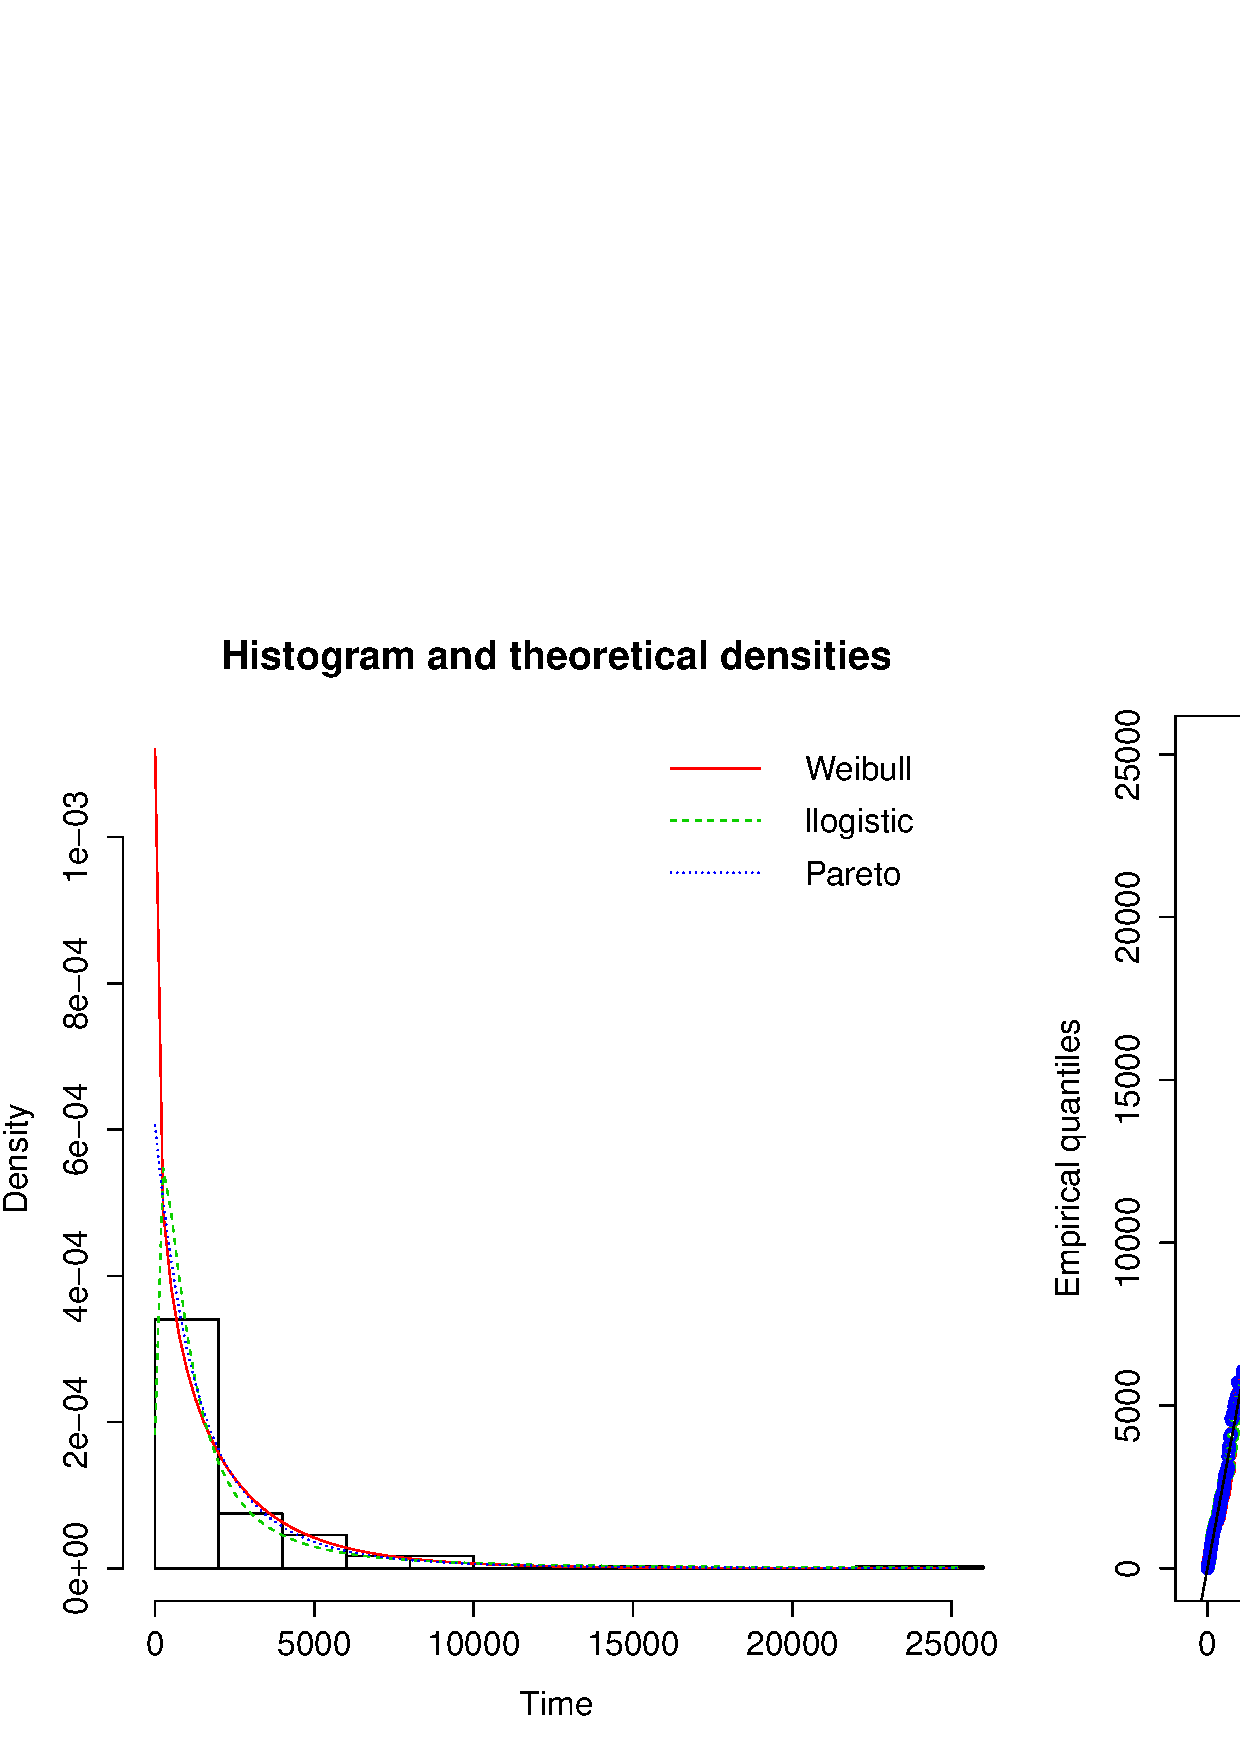
\includegraphics[width=6cm]{graph1.pdf} 
\caption{ Histogram of Outage Times (In Minutes) with fitted Log Normal Curve}
\end{center}
\label{fig:outagedistribution}
\end{figure}


\begin {table}
\caption {}
\begin{center}
\begin{tabular}{l*{3}{c}r} Statistic & Value 
\\ \hline Samples & 246
\\ Mean & 314.14
\\ Std Dev & 1414.43
\\ Median & 105
\\ Skew & 13.80
\\ Distribution & Log Normal
\\AD GoF Test (p) & 0.95
\end{tabular}
\end{center}
\end{table}


\subsection{Outage Component}

Fig. 2, 3 \& 4 and show the probability density function curves for outage events by component with a fitted Log Normal curve. These four categories total the full 246 outages. Due to the low number of samples (17) for the BSS \& Social category, the goodness of fit value should be treated with caution. \par

In each of the component categories, there is a degree of variability in relation to the mean outage times. Table III lists the summary statistics of outage events broken down by Component. E-Mail recorded the highest number of outages with 62\% of all outages, while Mixed, Collaboration and BSS-Social recorded 17\%, 14\% and 7\% respectively. 


\begin{figure}
\begin{center}
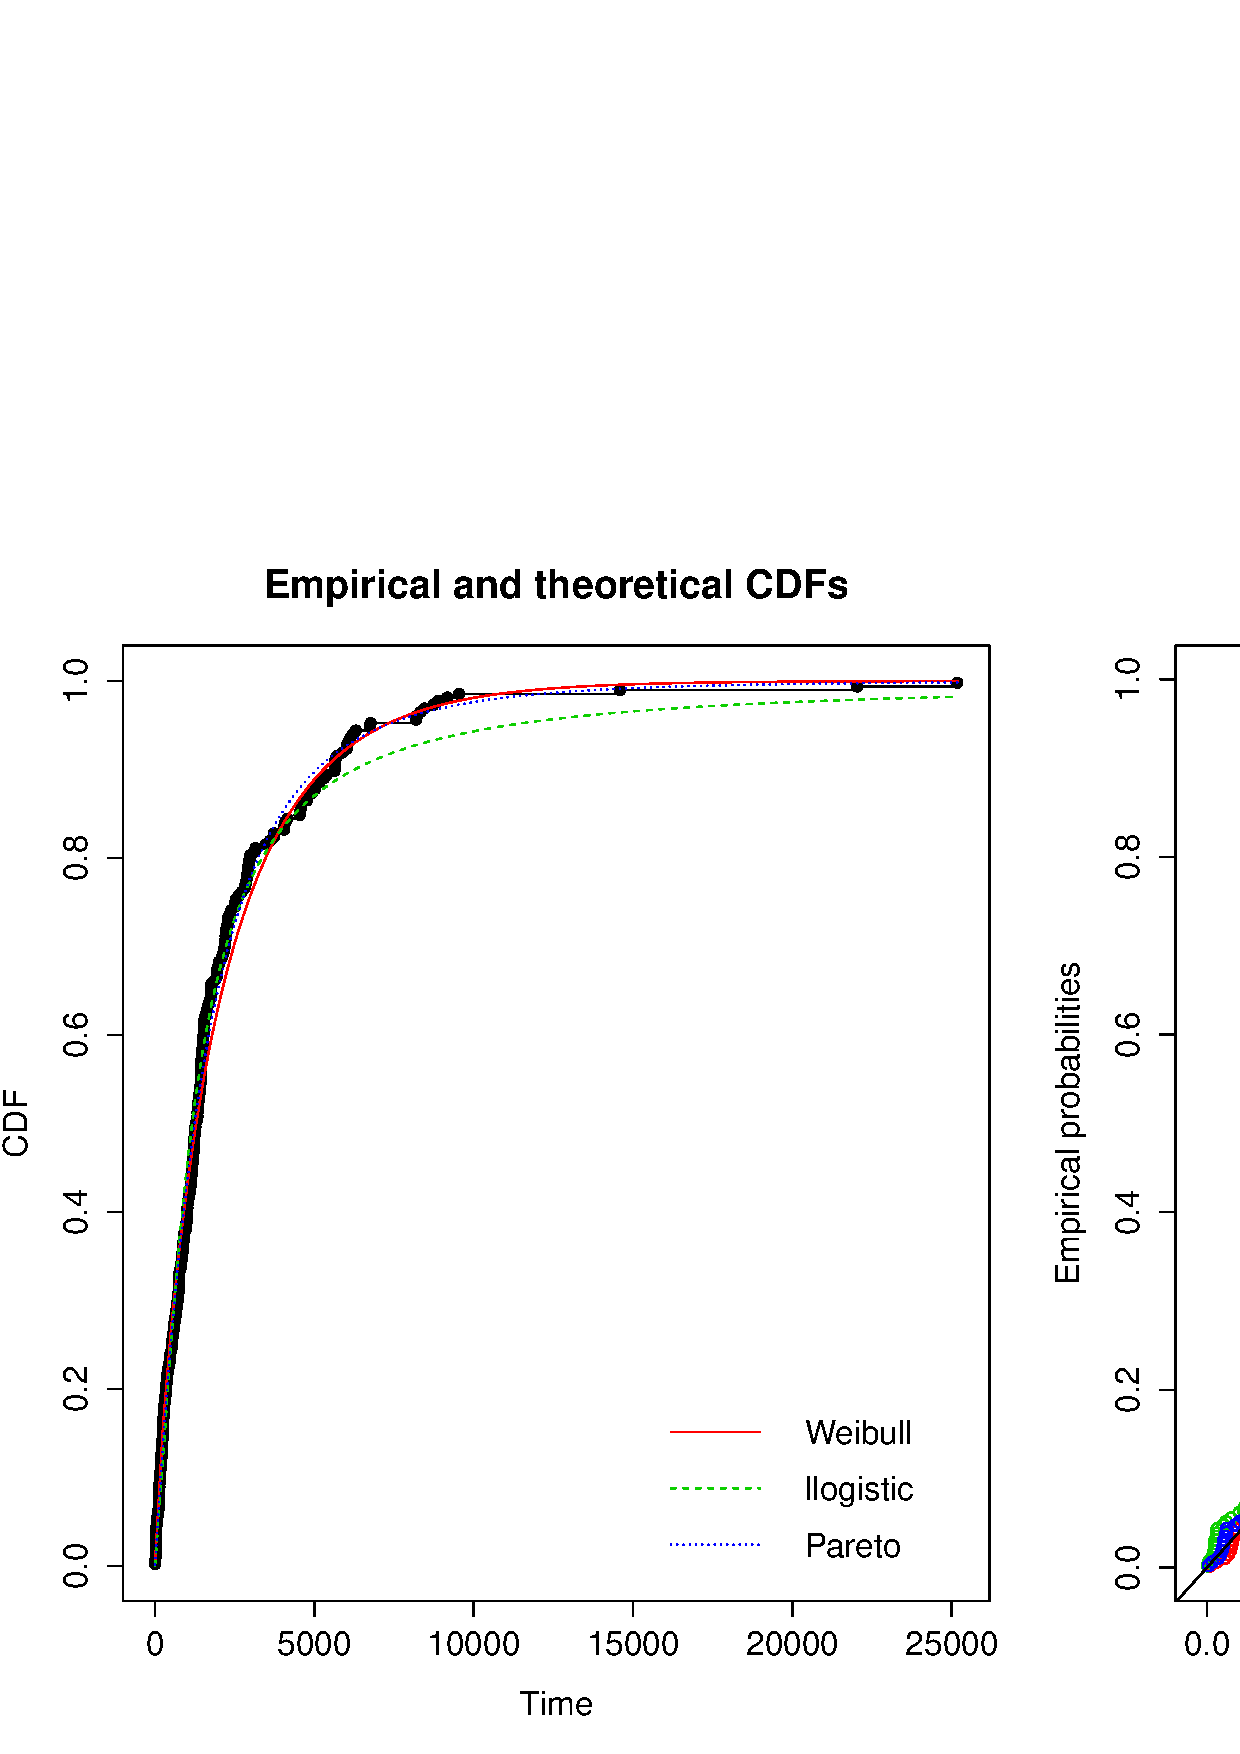
\includegraphics[width=6cm]{graph2.pdf} 
\caption{ Histogram of BSS-Social Times (In Minutes) with fitted Log Normal Curve}
\end{center}
\label{fig:outagedistribution}
\end{figure}


\begin{figure}
\begin{center}
\includegraphics[width=6cm]{graph3.pdf} 
\caption{ Histogram of Collaboration Times (In Minutes) with fitted Log Normal Curve}
\end{center}
\label{fig:outagedistribution}
\end{figure}



\begin{figure}
\begin{center}
\includegraphics[width=6cm]{graph4.pdf} 
\caption{ Histogram of E-Mail  Outage Times (In Minutes) with fitted Log Normal Curve}
\end{center}
\label{fig:outagedistribution}
\end{figure}

\begin{figure}
\begin{center}
\includegraphics[width=6cm]{graph5.pdf} 
\caption{ Histogram of Mixed Outage Times (In Minutes) with fitted Log Normal Curve}
\end{center}
\label{fig:outagedistribution}
\end{figure}



\begin {table}
\caption {}
%\caption {\% Field defects by impact} 
\begin{center}
\begin{tabular}{l*{3}{c}r} Statistic & BSS-Social & Collaboration & Email & Mixed
\\ \hline Samples & 16 & 34 & 152 & 43
\\ \% Samples & (7) & (14) & (62) & (17)
\\ Mean & 274.23 & 189 & 258.10 & 626.95
\\ Std Dev & 639.44 & 379.33 & 423.27 & 3260.78
\\ Median & 45	& 61.5 & 126.5 & 85
\\ Skew & 3.56	& 3.83 & 5.45 & 6.30
\\ Distribution & Log Normal & Log Normal & Log Normal  & Log Normal
\\AD GoF (p) & 0.69 & 0.62 & 0.99 & 0.64
\end{tabular}
\end{center}
\end{table}


\subsection{Outage Type}

Fig. 6 - 10 and show the probability density function curves for outage events by type with a fitted Log Normal curve. These five categories total the full 246-outage events. Due to the low number of samples (23) for the Hardware-Other category, the goodness of fit value should be treated with caution. \par

In each of the type categories, there is a degree of variability in the mean outage times. Table IV lists the summary statistics of outage events broken down by type. Configuration-Manual and Contention-Concurrency recorded the highest number of outages with 30\% and 26\% respectively. Network, Disaster Recovery and Hardware-Other categories recorded 20\%, 15\% and 9\% respectively. 

\begin{figure}
\begin{center}
\includegraphics[width=6cm]{graph6.pdf} 
\caption{ Histogram of Configuration-Manual Outage Times (In Minutes) with fitted Log Normal Curve}
\end{center}
\label{fig:outagedistribution}
\end{figure}

\begin{figure}
\begin{center}
\includegraphics[width=6cm]{graph7.pdf} 
\caption{ Histogram of Contention-Concurrency Outage Times (In Minutes) with fitted Log Normal Curve}
\end{center}
\label{fig:outagedistribution}
\end{figure}


\begin{figure}
\begin{center}
\includegraphics[width=6cm]{graph8.pdf} 
\caption{ Histogram of Disaster Recovery  Outage Times (In Minutes) with fitted Log Normal Curve}
\end{center}
\label{fig:outagedistribution}
\end{figure}

\begin{figure}
\begin{center}
\includegraphics[width=6cm]{graph9.pdf} 
\caption{ Histogram of Network Outage Times (In Minutes) with fitted Log Normal Curve}
\end{center}
\label{fig:outagedistribution}
\end{figure}

\begin{figure}
\begin{center}
\includegraphics[width=6cm]{graph10.pdf} 
\caption{ Histogram of Hardware-Other Outage Times (In Minutes) with fitted Log Normal Curve}
\end{center}
\label{fig:outagedistribution}
\end{figure}

\begin {table}
\caption {}
%\caption {\% Field defects by impact} 
\begin{center}
\begin{tabular}{l*{5}{c}r} Statistic & Configuration & Contention & Disaster & Network & Hardware
\\ & -Manual & -Concurrency &  Recovery & & -Other
\\ \hline \# Samples & 74 & 64 & 36 & 49 & 23
\\ \% Samples & 30 & 26 & 15 & 20 & 9
\\ Mean & 488.61 & 238.78 & 134.03 & 	314.59	& 243.44
\\ Std Dev & 2488.21	& 468.62	& 160.72	& 590.74	& 357.54
\\ Median & 114.5	& 86	& 72	& 145	& 91
\\ Skew & 8.28	& 3.69	& 2.33	& 5.30	& 2.11
\\ Distribution & Log Normal & Log Normal & Log Normal  & Log Normal & Log Normal
\\AD GoF (p) & 0.91 & 0.97 & 0.94 & 0.75 & 0.96
\end{tabular}
\end{center}
\end{table}


\subsection{Data Centre Location}

Fig. 12, 13 and 14 show the probability density function curves for outage events by data centre with a fitted Log Normal curve. These three categories total 238 events. A further 8 outages were found in all three data centres, however due to the low number of samples detailed analysis was not performed. Furthermore the researches felt it in was inappropriate to merge these eight samples into one of the existing data centre pools. \par

In each data centre there is variability in the mean outage times. Previously it was noted that Data Centre A, B and C are high, medium and low use respectively. Given the level of outage events in each data centre, the logical concept that higher usage results in more outages. However from the data set below this is the case for Data centre A, however Data centre C had more than double the outages than Data Centre B. \par

Table V lists the summary statistics of outage events broken down by data centre. Data Centre A recorded the highest number of outages with 65\% of all outages, while Data centre B and C recording 10\% and 22\% respectively. The remaining 3\% were from outages found in all thee data centres.

\begin{figure}
\begin{center}
\includegraphics[width=6cm]{graph11.pdf} 
\caption{ Histogram of Data Centre A Outage Times (In Minutes) with fitted Log Normal Curve}
\end{center}
\label{fig:outagedistribution}
\end{figure}

\begin{figure}
\begin{center}
\includegraphics[width=6cm]{graph12.pdf} 
\caption{ Histogram of  Data Centre B Outage Times (In Minutes) with fitted Log Normal Curve}
\end{center}
\label{fig:outagedistribution}
\end{figure}

\begin{figure}
\begin{center}
\includegraphics[width=6cm]{graph13.pdf} 
\caption{ Histogram of  Data Centre C Outage Times (In Minutes) with fitted Log Normal Curve}
\end{center}
\label{fig:outagedistribution}
\end{figure}


\begin {table}
\caption {}
%\caption {\% Field defects by impact} 
\begin{center}
\begin{tabular}{l*{3}{c}r} Statistic & Data Centre A & Data Centre B  & Data Centre C 
\\ \hline Samples & 160 & 24 & 54 
\\ \% Samples & 65 & 10 & 22
\\ Mean & 224.43	& 187.67	& 645.39
\\ Std Dev & 312.83	& 279.97	& 2961.09 
\\ Median & 113.5	& 89.5	& 79.5
\\ Skew & 2.93	& 2.89	& 6.67 
\\ Distribution & Log Normal & Log Normal & Log Normal  
\\AD GoF (p) & 0.99 & 0.99 & 0.31 
\end{tabular}
\end{center}
\end{table}






\section{Discussion}

Section IV provided an outline of outage events that were studied as part of our overall dataset, including distribution, component, type, data centre location and a comparison between detection time  and resolution time. The following section provides deeper analysis of the results. In each section references will be made to each research question asked in section III.

\subsection{Outage Distribution}

To answer the question how are the times of cloud outage events distributed, Fig. 1 and TABLE II clearly show that the distribution type is Log Normal. Of interest is the quality of the fit. An Anderson Darling goodness of fit test was conducted and a p value was found to be 0.947 with a test statistic of 0.287. In this case the hypothesis of whether the outage times are Log normally distributed cannot be rejected given the overwhelming evidence to the contrary.  \par

It is also worth noting that the mean outage time is approximately 314 minutes, which indicates that resolution of an outage in complex system architecture is a non-trivial task. Additionally with a standard deviation found to be approximately 1414 minutes and a skew value of 13.80, clearly indicated that there is a high level of dispersion within the dataset. \par

Given the nature of cloud computing new code updates and configuration changes are made on a regular basis. It is not uncommon for an enterprise to introduce changes or a monthly or bi-weekly basis. Therefore with this high level of system activity it is not unsurprising that outages can occur when least expected. If a state of the art outage tracking system were introduced, it would be interesting to determine as overall both process improvements were made coupled with underlying code stability to observe the overall affect on both the distribution type and shape. This would provide a concrete answer to questions such as: what impact do specific process improvements make to overall outage times? As a business where do resources need to be deployed to improve platform stability - Development, Operations or Quality Assurance? \par

\subsection{Outage Component}

Examining outages by component can given insight as to which component are likely to exhibit outages and whether these times vary by component. \par

Fig. 2 to 5 and TABLE III highlight that there is indeed variability in mean outages times across the components measured. Mixed components had the highest mean time with 626.95 minutes, followed by BSS-Social, Mail with 274.23 \& 258.10 respectively and finally Collaboration with 189 minutes. Indeed Mixed components also had the highest standard deviation and skew. This indicated firstly that mixed component outages take longer to resolve than single component issues, which makes sense given the level of remediation required. However in terms of overall outages the level of mixed component outages was 17\% of the overall total. It is also worth noting the number of outages in the e-mail category with 59\% is by far the highest contributor by component, yet the expected outage time is 258.10 minutes.  From closer inspection, the mean outage times for mixed component are due to a number of outages with high durations. \par

In all cases, each component class had a good fit to a Log Normal distribution, with the e-mail category fitting best with a p value of 0.995. However with a low sample count the goodness of fit values for the BSS-Social category should be treated with some caution. \par

Based on these results there are two areas of focus: first the quantities of outages related to the e-mail component and second the outage times to the mixed component outages. Tiger teams [ref] could be engaged to understand the root cause of both sets of issues. With knowledge gained through investigative techniques process improvements can be introduced which will allow deployment of crisis situation teams to other parts of the infrastructure. \par

\subsection{Outage Type}
Examining outages by type gives and deeper understanding of what types of problems are likely to cause an outage within a cloud infrastructure. Fig 6 ? 10 and TABLE IV provide this insight. \par

Configuration-Manual and Contention-Concurrency had the highest proportion of outages found with 30\% and 36\% respectively. While Network, Disaster Recovery and Hardware other had 20\%, 15\% and 9\% respectively. Significantly Configuration-Manual had the highest expected outage time with 488.61 minutes, with Network next highest with 314.59 minutes. Contention-Concurrency, Hardware and Disaster recovery had expected outages times of 238.78, 243.44 and 134.03 respectively. Finally the outage times of each category were fitted with a Log Normal distribution. In each case the hypothesis of whether a Log Normal distribution was a suitable distribution could not be rejected. However one caveat is that the Hardware-Other category had a low number of samples, so this result must be treated with caution. \par

Based on the above findings it is clear that issues related to Configuration-Manual contribute most to the overall number of outages but also take the longest to resolve.  Given the relative complexity of the overall cloud architecture it is apparent that a system of managed configuration changes is require. Firstly to ensure there is an audit trail of all changes made but secondly to ensure a level of pre-validation is done to ensure that harmful (extreme) values are rejected. Additionally tiger teams should also implement a system, which can monitor real-time configuration changes across the plurality of data centres.  \par

With any distributed system the network health plays an important role in system stability, while a data. Our network issues fell into two main categories: network congestion and temporal network outages. For congestion issues, business and operations teams need to define clear bandwidth capacity requirements to ensure that their infrastructure had the bandwidth to meet the demands of the existing user base and future subscription signings. Finally the underlying application and middleware stack should have additional resiliency added to ensure that temporal outages do not cause cascade failures, which can cause a single or multiple components to become unavailable once the network path has been restored. \par


\subsection{Data Centre Location}

Fig. 11 - 13 and TABLE V give insight into the outages by data centre. Discussed previously in section III, user concurrency varies by data centre. Data centre A (High Usage) had the highest number of outages with 65\% while Data centre B (Medium Usage) and Data centre C (Low Usage) had 10\% and 22\% respectively. A remaining 3\% of issues affected two or more data centres. Data Centre C had the highest mean outage time with 645.39 minutes, while data centre A \& B had mean outages times of 224.43 and 187.67 respectively. All three data centre outage times were modelled with a Log Normal distribution and both data centre A \& B were excellent fits with p values of 0.995 and 0.986 respectively. Data centre C faired worst in terms of fit with a p value of 0.316. Even with this value the hypothesis of whether a log normal distribution is a suitable fit cannot be rejected. \par

In some ways the above results are expected, it seems reasonably logical that a high use data centre would have the most outages logged due to the high level of activity, however even with all these outages the mean outage time is 224.43 minutes, which is approximately 90 minutes less than the overall mean. What appears somewhat counter intuitive is that data centre c has the second highest number of outages and the highest mean outage time. From closer inspection the mean outage times of data centre c are due to a number of outages with high durations. \par

In the context of software delivery to multiple data centres, the same code is release to each system. Clearly customers are impacted in different ways depending on which data centre is used. With this knowledge tiger teams can investigate in two areas. Firstly does the underlying customer use case of each data centre vary? Secondly a root and branch investigation of each data centre configuration should be conducted and compared for discrepancies, with specific focus on the e-mail component configuration. \par

\subsection{Detection time Vs Resolution time}

We outlined in section III that the overall outage time is divided further into two discrete units: The detection and resolution time. We discussed previously that a number of entries were removed from our analysis due to the having a value of 0. In the case of a 0 minute detection time, upon closer inspection these failures were flagged by internal operations teams, which in effect meant the time between first failure and resolution work, was immediate. In the case of a 0 minute resolution time, against these relate to issues that were raised internally. Operations times were working in parallel to upgrade a piece of infrastructure to prevent an failure, therefore when the failure event was flagged the new piece of infrastructure was in place to remediate the original issue when mean an immediate resolution due to the pre-emptive work. \par

Comparing the measures of location of both sets of untransformed data is readily apparent that it takes over twice as long for operations teams to become aware of a failure event than it does to resolve the problem once the failure is known. Additionally the dispersion within the detection times is high, a skew of 13.57 was computed. This may point to the quality of real-time monitoring solutions to detect failure events not only in the application and middle stack but also in the underlying data centre configuration and underlying network. Enhancing real-time anomaly detection may help reduce the detection time. We noted previously that e-mail, configuration-manual, and data centre a outages scored highest in each category. It is logical to assume that the operations and critical situation teams are engaged in resolving these issues over other types. By triangulation of outages on these three axes we now have a targets model for tiger teams to reduce repair time outcomes. \par

Finally it is worth commenting on the distribution type for both units. Fig. 14 and 15 show the distribution curves for both.  In the case of resolution time a lognormal curve was fitted and goodness of fit was value was computed to be 0.5. In this case the assumption of log normal distribution for resolution times cannot be rejected. This finding complements existing work related to the usefulness of the log normal distribution to model repair times of maintainable systems. In the case of detection time a lognormal curve was fitted however a goodness of fit test was conducted and a p-value of 0.01 was computed. In this case there was moderate evidence against the use of log normal to model detection times. Given the level of skew within the detection time data a log transformation was applied. Subsequently a log normal distributed was fitted and a goodness of fit test conducted. A p-value was calculated to be 0.46. . In this case the assumption of log normal distribution for log transformed detection times cannot be rejected. While detection times are a function of the overall outage time, this finding suggests that detection times themselves have wider spread of values than resolution times and should be treated a special case in itself. \par



\vspace{-1mm}
\section{Conclusion}
Previous studies have shown that shown that Cloud Outages are an infrequent occurrence. Additionally that the Log normal distribution is a useful tool for modelling repair times in mechanical and electronic maintainable systems. \par

The purpose of this study was to examine the duration of outage events within a Cloud based application platform. It was found that the log normal distribution is a useful model for modelling repair times for SaaS applications. The findings of this study support previous studies particularly in the area of system reliability and repair times. \par

This work provides a more comprehensive study in relation to how outage times can vary between the types of outage, the component involved and the data centre in use at the time of outage. \par

In future SMEs can assess their outage data to understand the core issues that effect their underlying service platform. A specific operations framework can then be developed to allow the SME to focus on specific parts of their architecture or business process, which impede high value growth. Likewise usage of framework on an iterative basis can be used to by SMEs to set achieve realistic remediation targets. \par

In future work we shall assess our framework in conjunction with the time between outage events to understand how best operations teams can be deployed where parallel outage events occur.  \par

% An example of a floating figure using the graphicx package.
% Note that \label must occur AFTER (or within) \caption.
% For figures, \caption should occur after the \includegraphics.
% Note that IEEEtran v1.7 and later has special internal code that
% is designed to preserve the operation of \label within \caption
% even when the captionsoff option is in effect. However, because
% of issues like this, it may be the safest practice to put all your
% \label just after \caption rather than within \caption{}.
%
% Reminder: the "draftcls" or "draftclsnofoot", not "draft", class
% option should be used if it is desired that the figures are to be
% displayed while in draft mode.
%
%\begin{figure}[!t]
%\centering
%\includegraphics[width=2.5in]{myfigure}
% where an .eps filename suffix will be assumed under latex, 
% and a .pdf suffix will be assumed for pdflatex; or what has been declared
% via \DeclareGraphicsExtensions.
%\caption{Simulation Results}
%\label{fig_sim}
%\end{figure}

% Note that IEEE typically puts floats only at the top, even when this
% results in a large percentage of a column being occupied by floats.


% An example of a double column floating figure using two subfigures.
% (The subfig.sty package must be loaded for this to work.)
% The subfigure \label commands are set within each subfloat command, the
% \label for the overall figure must come after \caption.
% \hfil must be used as a separator to get equal spacing.
% The subfigure.sty package works much the same way, except \subfigure is
% used instead of \subfloat.
%
%\begin{figure*}[!t]
%\centerline{\subfloat[Case I]\includegraphics[width=2.5in]{subfigcase1}%
%\label{fig_first_case}}
%\hfil
%\subfloat[Case II]{\includegraphics[width=2.5in]{subfigcase2}%
%\label{fig_second_case}}}
%\caption{Simulation results}
%\label{fig_sim}
%\end{figure*}
%
% Note that often IEEE papers with subfigures do not employ subfigure
% captions (using the optional argument to \subfloat), but instead will
% reference/describe all of them (a), (b), etc., within the main caption.


% An example of a floating table. Note that, for IEEE style tables, the 
% \caption command should come BEFORE the table. Table text will default to
% \footnotesize as IEEE normally uses this smaller font for tables.
% The \label must come after \caption as always.
%
%\begin{table}[!t]
%% increase table row spacing, adjust to taste
%\renewcommand{\arraystretch}{1.3}
% if using array.sty, it might be a good idea to tweak the value of
% \extrarowheight as needed to properly center the text within the cells
%\caption{An Example of a Table}
%\label{table_example}
%\centering
%% Some packages, such as MDW tools, offer better commands for making tables
%% than the plain LaTeX2e tabular which is used here.
%\begin{tabular}{|c||c|}
%\hline
%One & Two\\
%\hline
%Three & Four\\
%\hline
%\end{tabular}
%\end{table}


% Note that IEEE does not put floats in the very first column - or typically
% anywhere on the first page for that matter. Also, in-text middle ("here")
% positioning is not used. Most IEEE journals/conferences use top floats
% exclusively. Note that, LaTeX2e, unlike IEEE journals/conferences, places
% footnotes above bottom floats. This can be corrected via the \fnbelowfloat
% command of the stfloats package.




% conference papers do not normally have an appendix


% use section* for acknowledgement
%\section*{Acknowledgment}


%The authors would like to thank...





% trigger a \newpage just before the given reference
% number - used to balance the columns on the last page
% adjust value as needed - may need to be readjusted if
% the document is modified later
%\IEEEtriggeratref{8}
% The "triggered" command can be changed if desired:
%\IEEEtriggercmd{\enlargethispage{-5in}}

% references section

% can use a bibliography generated by BibTeX as a .bbl file
% BibTeX documentation can be easily obtained at:
% http://www.ctan.org/tex-archive/biblio/bibtex/contrib/doc/
% The IEEEtran BibTeX style support page is at:
% http://www.michaelshell.org/tex/ieeetran/bibtex/
\vspace{-2mm}
\bibliographystyle{IEEEtran}
% argument is your BibTeX string definitions and bibliography database(s)
\bibliography{socialtest}
\vspace{-5mm}
%
% <OR> manually copy in the resultant .bbl file
% set second argument of \begin to the number of references
% (used to reserve space for the reference number labels box)


% that's all folks
\end{document}


